\documentclass{article}

\usepackage{graphicx}
\usepackage{subfig}
\usepackage{amsmath}
%\usepackage{amsmath,rotating}

\title{Laminar, Two-dimensional Channel Flow}

\date{}

\begin{document}

\maketitle

\section{Introduction}
This case provides a description for two-dimensional channel flow
with constant properties, and a constant pressure gradient.

\section{Domain}
The two-dimensional geometry for this tutorial is captured in 
Figure~\ref{fig:geom} where the rectangular domain is defined by the 
height, $H$, and length, $L$. The streamwise and vertical velocity are 
defined as $u_x$ and $u_y$, respectively.

The top and bottom surfaces are no-slip wall boundary specifications with $u_x = u_y = 0$,
while the left and right surfaces are open boundaries in which a static 
pressure is supplied. Zero normal gradients are applied to the open boundary. In 
absence of any external body forces, the flow is 
aligned to the x-axis and is strictly a function of the vertical-dimension, $y$,
i.e., $u_x = f(y)$.

\begin{figure}[!htbp]
  \centering
  {
   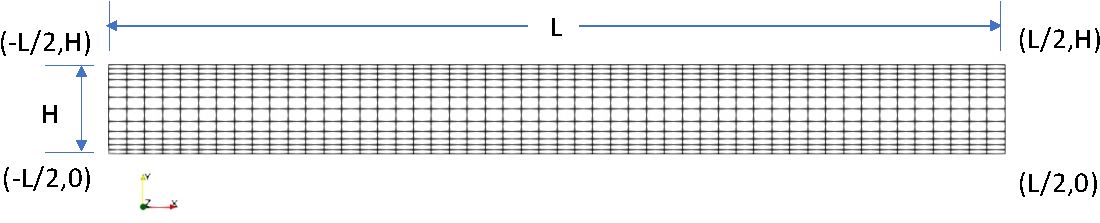
\includegraphics[height=1.0in]{images/2d_quad4_channel_geom.pdf}
  }
  \caption{Two-dimensional channel flow in which the height is unity and length, 10.}
  \label{fig:geom}
\end{figure}

\section{Theory}
The variable-density low-Mach equation set is defined by the continuity and momentum equation,

\begin{align}
  \frac {\partial \rho }{\partial t} + \frac{ \partial \rho u_j}{\partial x_j} = 0.
\label{eq:contEq}
\end{align} 

\begin{align}
  \frac {\partial \rho u_i }{\partial t} + \frac{ \partial \rho u_j u_i}{\partial x_j} 
-\frac{\partial \sigma_{ij}}{\partial x_j} = 0.
\label{eq:momEq}
\end{align}
%
In the above equation, $\rho$ is the fluid density and $u_j$ is the fluid velocity. 
The stress tensor is provided by
\begin{align}
\sigma_{ij}  = 2 \mu S^*_{ij} - P \delta_{ij},
\end{align}
%
where the traceless rate-of-strain tensor is defined as
\begin{align}
S^*_{ij}  = S_{ij} - \frac{1}{3} \delta_{ij} S_{kk} \nonumber
		     = S_{ij} - \frac{1}{3} \frac{\partial  u_k }{\partial x_k}\delta_{ij}.
\end{align}
In a low-Mach flow, the above pressure, $P$, is the perturbation about the thermodynamic
pressure, $P^{th}$. 

\subsection{Analytical Velocity Profile}
Given the assumptions provided in the introduction, the streamwise velocity equation reduces to,

\begin{align}
  \frac{d P}{dx} = \mu \frac{d^2 u_x}{dy^2}.
\label{eq:simpEq}
\end{align}
This equation can be integrated twice to obtain,

\begin{align}
  u_x(y) = \frac{1}{\mu}\frac{d P}{dx} \frac{y^2}{2} + k_1 y + k_2,
\label{eq:simpEqWithK}
\end{align}
where $k_1$ and $k_2$ are constants of integration that are obtained through the 
application of boundary conditions, $u_x(y=0) = 0$ and  $u_x(y=H) = 0$. Therefore,
the final expression for the streamwise velocity is,

\begin{align}
  u_x(y) = \frac{1}{2 \mu}\frac{d P}{dx}\left[ y^2 - Hy \right].
\label{eq:simpleEqWithoutK}
\end{align}

The above equation can be used to determine the vertical location at which 
the maximum velocity is found via solving $\frac{du_x}{dy} = 0$, or $u^{max}_x$ 
occurs at $H/2$. The functional form for the maximum velocity is,

\begin{align}
  u^{max}_x = \frac{1}{8 \mu}\frac{d P}{dx}H^2.
\label{eq:uMax}
\end{align}

\section{Results}
Let us test a simulation in which the Reynolds number based on wall friction
velocity, $u^\tau$, and half-channel height $H/2$, is ten: $Re^\tau$ = 10.
By constraining the Reynolds number, wall friction velocity, and density, 
the consistent viscosity is obtained via,

\begin{align}
  \mu = \frac{\rho u^\tau H}{2 Re^\tau}.
\label{eq:muForm}
\end{align}

To obtain the required pressure gradient, we exercise the relationship,

\begin{align}
  u^\tau = \sqrt{\frac{\tau_w}{\rho}},
\label{eq:tauWall}
\end{align}
along with global momentum balance,
%
\begin{align}
\int \frac{dP}{dx} dV = \int \tau_w dA,
\label{eq:balance}
\end{align}
with $dV = LH$ and $dA = 2L$, to obtain the relationship between
required pressure gradient and wall shear stress, $\frac{dP}{dx} = 2\tau_w$.

\subsection{Simulation Specification and Results}

Arbitrarily setting the density and wall friction velocity to unity, 
along with enforcing the height to be unity, provides a viscosity of $1/20$.
Moreover, the required pressure gradient given our channel length of 10 is
2. The mesh exercised activates a Quad4 topology, thereby exercising a
linear underlying basis that yields a nominal second-order spatial accurate
simulation.

In Figure~\ref{fig:results}, results are provided for the specifications
provided above.

\begin{figure}[!htbp]
  \centering
  {
   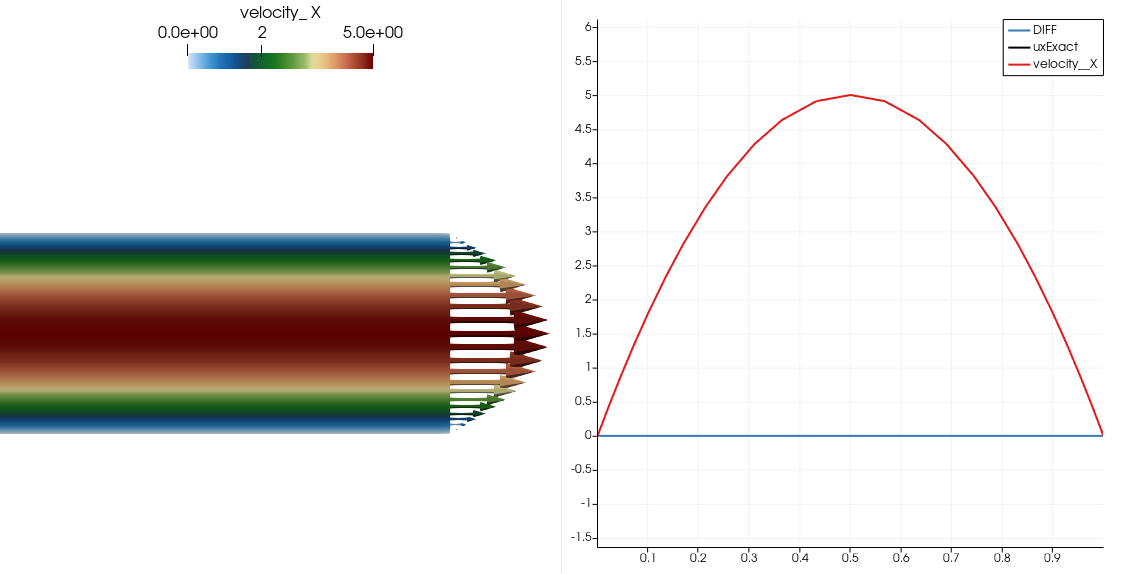
\includegraphics[height=2.0in]{images/2d_quad4_channel_results.png}
  }
  \caption{Velocity shadings and profile for the $Re^\tau = 10$ case.}
  \label{fig:results}
\end{figure}

\section{Discussion Points}

There are several interesting activities associated with this sample case including
the following:

\begin{itemize}
	\item Ensure that derivation of Equation~\ref{eq:simpleEqWithoutK} is clear.
	\item Ensure that derivation of Equation~\ref{eq:uMax} is clear.
	\item Ensure that derivation of Equation~\ref{eq:balance} and the expression
           $\frac{dP}{dx} = 2\tau_w$ is clear.
	\item Explore the mesh and input file specifications associated with this case.
	\item In Figure~\ref{fig:results}, it is noted that the difference between
          the analytical and simulation result is zero. When you run the two mesh resolutions provided, 
          does this finding hold? Why is this?
        \item Probe all degree-of-freedom results, i.e., velocity and pressure. What is of interest?
        \item When the simulation is run and wall shear stress is provided in the output file,
          what is the value? What are your findings?
\end{itemize}

\end{document}
